\documentclass[a4paper,10pt-]{article}

\usepackage{graphicx}
\usepackage{tabularx}
\usepackage{listings}
\usepackage[normalem]{ulem}

\lstset{ %
language=HTML,    % choose the language of the code
basicstyle=\footnotesize,       % the size of the fonts that are used for the code
numbers=left,       % where to put the line-numbers
numberstyle=\footnotesize,      % the size of the fonts that are used for the line-numbers
stepnumber=1,      % the step between two line-numbers. If it is 1 each line will be numbered
numbersep=5pt,      % how far the line-numbers are from the code
showspaces=false,   % show spaces adding particular underscores
showstringspaces=false,         % underline spaces within strings
showtabs=false,     % show tabs within strings adding particular underscores
frame=single,           % adds a frame around the code
tabsize=2,          % sets default tabsize to 2 spaces
captionpos=b,           % sets the caption-position to bottom
breaklines=true,        % sets automatic line breaking
breakatwhitespace=false,    % sets if automatic breaks should only happen at whitespace
escapeinside={\%*}{*)}          % if you want to add a comment within your code
}


\begin{document}

\title{Getting started with \emph{ivml.js}}
\author{J. Gentile and A. Meyers}

\maketitle

\section{Getting Started}

IVML, the Interactive Visualization Markup Language, is a JavaScript library that leverages popular JavaScript technologies Angular, D3 and JQuery to enable developers to quickly implement interactive data visualizations in a browser.
It has predefined a collection of embeddable Angular directives that bind to underlying
JavaScript objects. Let's demonstrate its functionality by quickly drawing this
graph:

\begin{figure}[!htb]
\centering
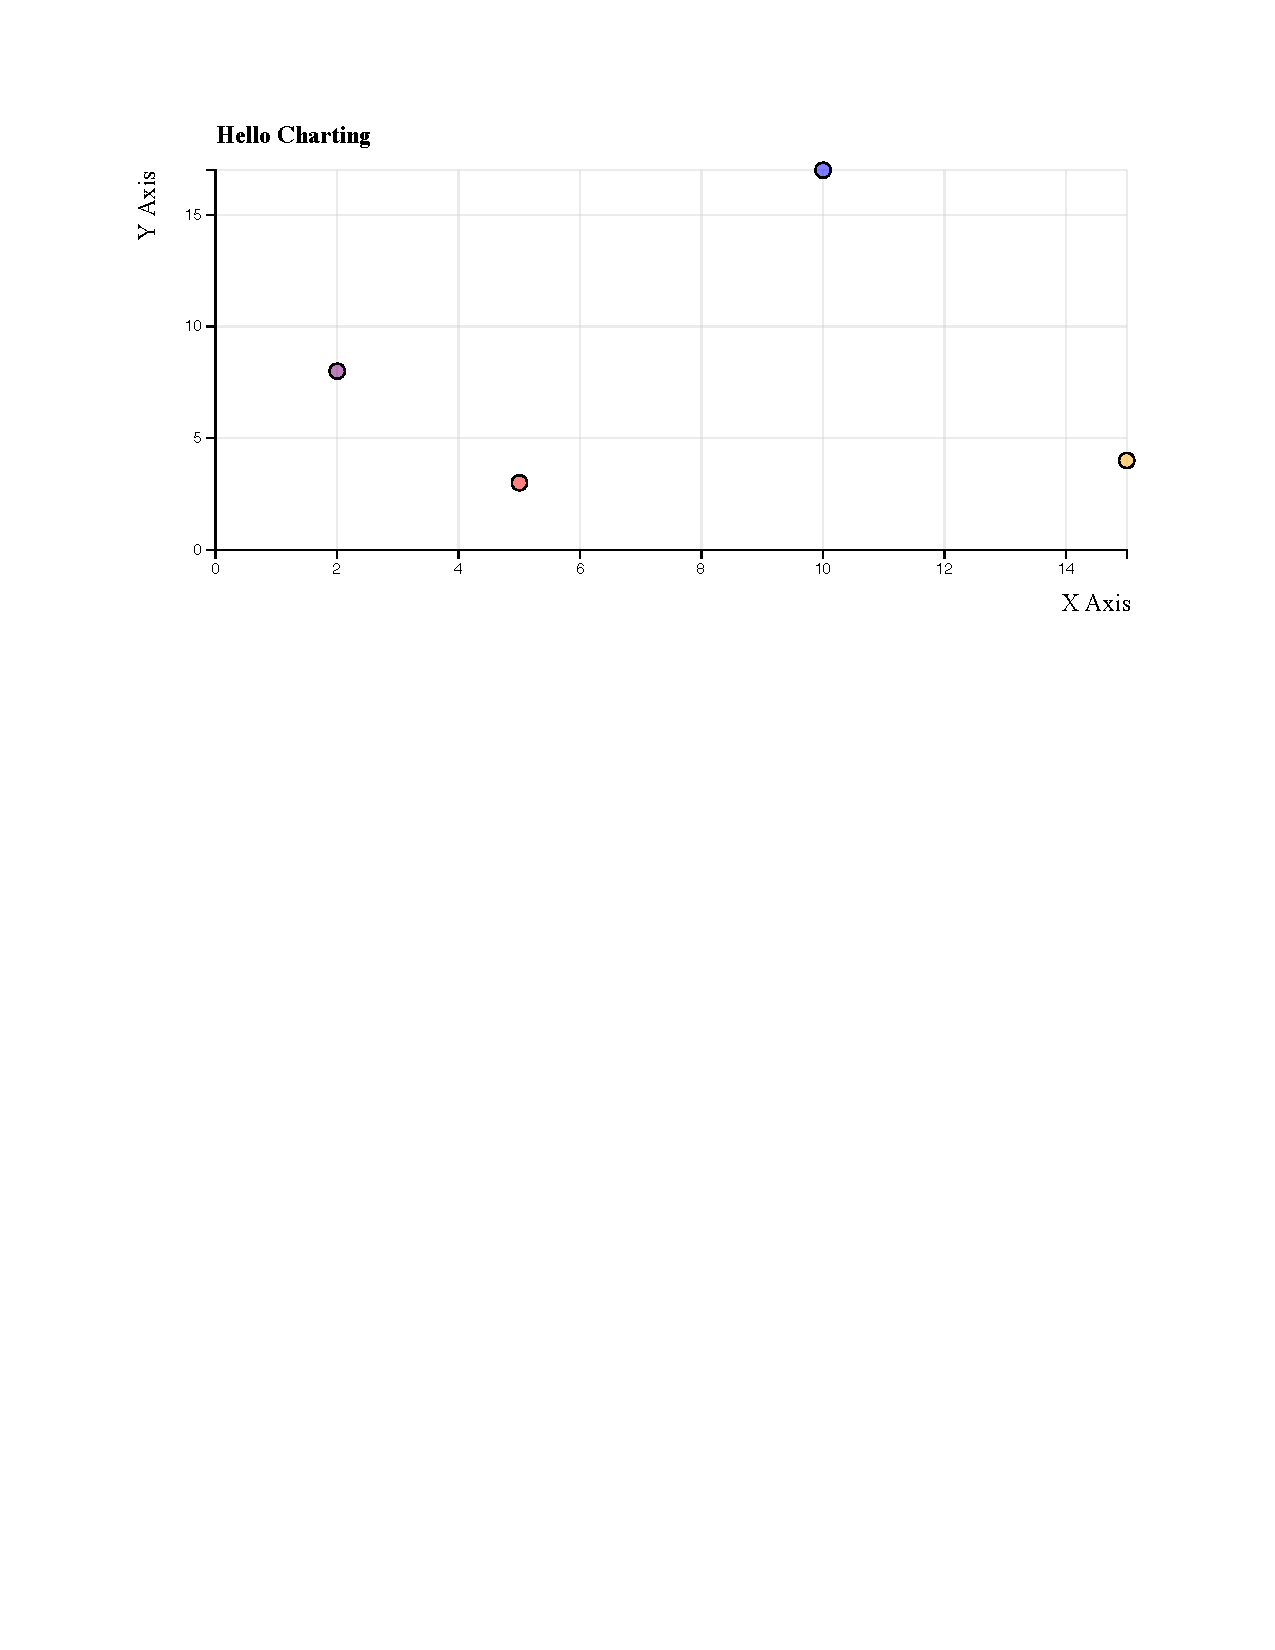
\includegraphics[scale=.6]{Images/HelloWorld.pdf}
\label{scatterplot}
\end{figure}

\noindent The code for generating this plot is listed below:

\lstset{language=HTML,label=ivml}

\begin{lstlisting}
<!DOCTYPE html>
<html>
<meta charset="utf-8">
<script type="text/javascript" src="./vendor/angular/angular.js"></script>
<script type="text/javascript" src="./vendor/d3/d3.js"></script>
<script type="text/javascript" src="./vendor/ivml/ivml.0.5.0.js"></script>

<body ng-app="app">
    <div ng-controller="controller">
        <div>
            <plot height="250" width="600" plot-label-text="'Hello Charting'" yaxis-label-text="'Y Axis'" xaxis-label-text="'X Axis'" xmin="0" xmax="xmax" yticks="5" ymin="0" ymax="ymax">
                <points data="data" yfunction="y" xfunction="x" fill='cfunc' radius="5" fill-opacity="0.5"
                        stroke="'black'">
                </points>
            </plot>
        </div>
    </div>
</body>
<script>
angular.module('app',['ivml'])
        .controller('controller',function($scope){
            $scope.data = [[5,3], [10,17], [15,4], [2,8]];
            $scope.xmax = d3.max($scope.data, function(d) { return d[0]; });
            console.log($scope.data)
            console.log($scope.xmax)
            $scope.ymax = d3.max($scope.data, function(d) { return d[1]; });
            $scope.x = function(d){
                return d[0];
            }
            $scope.y = function(d){
                return d[1];
            }
            $scope.cfunc = function(d,i){
                var c = ['red', 'blue', 'orange', 'purple' ]
                return c[i]
            }
        })
</script>
</html>
\end{lstlisting}

\noindent There are at least three things you will probably notice. First,  a couple of HTML tags look unfamiliar on lines 11 and 12 ({\tt <plot>}, {\tt <points>}), these directives are provided by IVML. Additionally, there is some \emph{angular.js} boilerplate code (lines 20, 21, and the {\tt \$scope} variable). Finally, various properties are defined on the {\tt \$scope} object. The next sections provide detail on graphing by directives and data management in \emph{angular.js}.

\subsection{Graphing by IVML Directive}

IVML provides a set of Angular directives to make graphing very easy. There are three types of these, charts, visual elements, and groups. Charts are high-level directives describing the canvas that visual elements are plotted on. Visual elements are graphics that represent data. In the provided example, the {\tt plot} directive describes the axes while {\tt points} represent the data for plotting. Groups are collections of visual elements that are necessary for generating some plots.

This approach allows us to embed an arbitrary number of visual elements inside a chart so it's easy to have points, line segments, error bars, and rectangles on the same plot. Each visual element can bind to data so expressive and custom graphs can be quickly generated with sets of simple visual elements.

Directives are configured by their attributes. In {\tt plot}, the attributes configure the plotting canvas and axes. Four of the attributes are constant values (attributes surrounded by {\tt ' '}), while the value of {\tt xmaximum} and {\tt ymaximum} corresponds to variables in the JavaScript. 

Some plots require visual elements to be part of a group. For example, collections of data in a bar graph should be centered around values on a nominal axis. IVML provides group directives for this purpose. Consider this code snippet from an HTML body:

\lstset{language=HTML,label=ivml}

\begin{lstlisting}
<plot xaxis-label-text="'Rects_x'" yaxis-label-text="' Rects y'"  xordinal-domain="odomain" yminimum="'-2'" ymaximum="2"  height="'200'" width="'200'">
      <bar-group padding="'2'" type="type">
          <bar data="data1" value-function="'/m'" position-function="'/o'" fill="'blue'" width="'4'"></bar>
          <bar data="data2" value-function="'/m'" position-function="'/o'" fill="'blue'" width="'4'"></bar>
          <bar data="data3" value-function="'/m'" position-function="'/o'" fill="'blue'" width="'4'"></bar>
      </bar-group>
</plot>

\end{lstlisting}

\noindent Notice there are multiple {\tt <bar>} tags in a {\tt <bar-group>}. Each {\tt <bar>} is associated with a unique data set but the position of each visual element will depend on other element positions so they must be grouped. 

\subsection{Designing with \emph{angular.js}}

IVML leverages \emph{angular.js} to define its controllers and directives because interactive data visualization are web applications. \emph{angular.js} is a `model-view-whatever' framework that allows you to develop very powerful web applications. We will cover just enough \emph{angular.js} to give us an understanding of what is going on in our example code but we recommend looking into \emph{angular.js} to learn all it can do. 

Notice on lines {\tt 8} and {\tt 9} there are {\tt ng-*} attributes in the {\tt div}s. These are defining the context of the embedded code for \emph{angular.js}. Our application is called {\tt app}; our controller is {\tt controller}; and we define those in lines {\tt 20} and {\tt 21}. Note that the controller is defined with a function that takes a {\tt \$scope} variable. 

Variables referenced in the {\tt ng-controller} HTML context are in the ``scope" so {\tt xmaximum="xmax"} means the {\tt xmaximum} attribute for the chart will be equal to {\tt \$scope.xmax}. The controller script defines the values referenced by IVML directives and when the referenced values change, the charts will automatically update. We define {\tt \$scope.data} and set it as the data attribute in {\tt points} so every time {\tt \$scope.data} is changed, the {\tt points} will update to reflect the new data values.

\subsection{Role of Callback Functions}

Notice that there are three functions described in the controller as members of the {\tt \$scope} object, {\tt x(d)}, {\tt y(d)}, and {\tt cfunc(d,i)}. These functions are given as the {\tt xfunction}, {\tt yfunction}, and {\tt fill} of {\tt points}. Points are drawn by adding {\tt circle} elements to the DOM and each element is given a set of attributes defined in the directive. When attribute values are given as callback functions, IVML passes the data object along with its index or key to the function and the returned value should be appropriate for the attribute (i.e. colors or numbers when necessary). 

The data being plotted is an array of arrays ({\tt \$scope.data}) so each element in the higher-level array represents each point. The accessor for the x position returns the first element of a data object, and the y position returns the second element. The fill of a point is dependent on its data's position in the list. Any visual element attribute can be passed in as a callback function except for {\tt data}. This should be familiar to users who know \emph{d3.js} (in fact, IVML uses \emph{d3.js} to bind data to DOM elements).

IVML has a construct to simplify callback functions that just return the value at an index or key. In the first example, {\tt \$scope.x(d)} and {\tt \$scope.y(d)} just returned the value at index {\tt 0} and {\tt 1}. This can be simplified an attribute a string with '/' as the leading character followed by the index or key. Therefore, on line 12, {\tt yfunction="y"} can be replaced with {\tt yfunction="'/1'"} and  the declaration of {\tt \$scope.y} can be removed. 

\subsubsection{Event Callbacks} 

IVML supports several events for when the user may mouse-over, mouse-out or click on a visual object. Callback functions for these events be set as an attribute. IVML will call event functions with three parameters: the data, index and DOM element (abbreviated as {\tt d,i,e}). Element properties can be changed by JavaScript methods (inkling d3 and jQuery functions). The examples directory provides samples of these events in action. 




\section{Documentation}

This section will describe the attributes and directives provided by IVML in detail. Recall that there are three types of directives, charts, visual elements, and groups. Visual objects need to be in a chart and groups are collections of visual objects. 

\subsection{\emph{ivml}, \emph{svg}, and \emph{event} Attributes}


Visual elements have three types of attributes: \emph{ivml}, \emph{svg}, and \emph{event}. In general, the data attribute in \emph{ivml} will point to a JavaScript object and the accessors will be javascript functions. \emph{svg} attributes can be constant values (surrounded by {\tt ''} or callback functions. \emph{event} attributes must be callback functions and the parameters are the data, index and DOM element. 

\begin{description}
\item[\emph{ivml attributes}]{are required by the toolkit and generally relate to the data and accessor routines required for rendering data in the correct position on a chart. }

\item[\emph{svg} attributes]{directly map to the svg attributes of visual elements so any formats or units recognized by the browser can be utilized.}

\item[\emph{event} attributes]{are functions that are called when a specified event occurs on a data object. The callback function's parameters are the data, key and DOM element .}

\end{description}

\subsection{How to Read the Directive Pages}

Each IVML directive is documented on the following pages. We provide a brief description, define the directive's type and list its attributes. \uline{An underlined attribute means it's required by the directive.} Examples for each directive's usage can be found in the accompanying files.

\clearpage \noindent \hrulefill
\subsection*{{\tt <plot>}}
\hrulefill\newline
 Cartesian chart with x and y axes.
\subsection*{\emph{ivml attributes}}
\begin{description}
\item[yodomain:]{array of nominal values for discrete y axes (overrides ymin, ymax, yticks)}
\item[xaxis-tick-size:]{tick size for x axis}
\item[xgridlines-visibility:]{visibility for x axis gridlines}
\item[ygridlines-stroke:]{stroke color for y axis gridlines}
\item[yaxis-truncate-ending:]{string to append to end of y axis text truncated due to exceeding yaxis-text-max-width}
\item[ygridlines-fill:]{fill color for y axis gridlines}
\item[margin-right:]{size in pixels of the right margin}
\item[height:]{height in pixels of the plot area}
\item[brush-stroke:]{stroke color for brush}
\item[xgridlines-stroke:]{stroke color for x axis gridlines}
\item[margin-left:]{size in pixels of the left margin}
\item[xmin:]{minimum value of the x axis}
\item[xaxis-label-text:]{x axis label}
\item[ymin:]{minimum value of the y axis}
\item[yaxis-tick-size:]{tick size for x axis}
\item[xgridlines-shape-rendering:]{shape rendering for x axis gridlines}
\item[xgridlines-fill:]{fill color for x axis gridlines}
\item[brush-fill-opacity:]{fill opacity for brush}
\item[ymax:]{maximum value of the y axis}
\item[ytick-format-function:]{formatter for y axis tick labels}
\item[yaxis-shape-rendering:]{shape rendering for y axis}
\item[margin-bottom:]{size in pixels of the bottom margin}
\item[xticks:]{number of tick marks to be shown on continuous x axis}
\item[width:]{width in pixels of the plot area}
\item[brush-fill:]{fill color for brush}
\item[ygridlines-opacity:]{opacity for y axis gridlines}
\item[brush-shape-rendering:]{shape rendering brush}
\item[plot-label-font-color:]{font color of the main label of the plot}
\item[yaxis-stroke:]{stroke color for y axis}
\item[xaxis-font-color:]{font color for x axis}
\item[yaxis-visibility:]{visibility value for y axis}
\item[plot-background:]{background color of the plot area}
\item[yaxis-font-size:]{font size for y axis}
\item[xaxis-text-max-width:]{maximum width of x axis text in pixels}
\item[xaxis-fill:]{fill color for x axis}
\item[xaxis-visibility:]{visibility value for x axis}
\item[ygridlines-visibility:]{visibility for y axis gridlines}
\item[xaxis-truncate-ending:]{string to append to end of x axis text truncated due to exceeding xaxis-text-max-width}
\item[background:]{background color of the entire element}
\item[xtick-format-function:]{formatter for x axis tick labels}
\item[ygridlines-shape-rendering:]{shape rendering for y axis gridlines}
\item[xaxis-shape-rendering:]{shape rendering for x axis}
\item[yaxis-font-color:]{font color for y axis}
\item[brush-clear-on-redraw:]{set to true if brush should clear when plot is redrawn}
\item[plot-label-font-size:]{font size of the main label of the plot}
\item[yaxis-font-family:]{font family for y axis}
\item[xodomain:]{array of nominal values for discrete x axes (overrides xmin, xmax, xticks)}
\item[xaxis-font-size:]{font size for x axis}
\item[yaxis-label-text:]{y axis label}
\item[xaxis-font-family:]{font family for x axis}
\item[yaxis-fill:]{fill color for y axis}
\item[margin-top:]{size in pixels of the top margin}
\item[plot-label-text:]{text for the main label of the plot}
\item[yaxis-text-max-width:]{maximum width of y axis text in pixels}
\item[xmax:]{maximum value of the x axis}
\item[yticks:]{number of tick marks to be shown on continuous y axis}
\item[xgridlines-opacity:]{opacity for x axis gridlines}
\item[xaxis-stroke:]{stroke color for x axis}
\end{description}
\subsection*{\emph{event attributes}}
\begin{description}
\item[ybrushstart:]{function that will be called when the vertical brush starts.  Will pass the d3.svg.brush element of the plot as the first parameter.}
\item[ybrush:]{function that will be called when the vertical brush is brushed.  Will pass the d3.svg.brush element of the plot as the first parameter.}
\item[xbrushend:]{function that will be called when the horizontal brush ends.  Will pass the d3.svg.brush element of the plot as the first parameter.  Setting the function disables ybrushstart, ybrush, ybrushend.}
\item[xbrushstart:]{function that will be called when the horizontal brush starts.  Will pass the d3.svg.brush element of the plot as the first parameter.  Setting the function disables ybrushstart, ybrush, ybrushend.}
\item[xbrush:]{function that will be called when the horizontal brush is brushed.  Will pass the d3.svg.brush element of the plot as the first parameter.  Setting the function disables ybrushstart, ybrush, ybrushend.}
\item[ybrushend:]{function that will be called when the vertical brush ends.  Will pass the d3.svg.brush element of the plot as the first parameter.}
\item[brush:]{function that will be called when the two dimensional brush is brushed.  Will pass the d3.svg.brush element of the plot as the first parameter.  Setting the function disables xbrushstart, xbrush, xbrushend, ybrushstart, ybrush, ybrushend.}
\item[brushend:]{function that will be called when the two dimensional brush ends.  Will pass the d3.svg.brush element of the plot as the first parameter.  Setting the function disables xbrushstart, xbrush, xbrushend, ybrushstart, ybrush, ybrushend.}
\item[brushstart:]{function that will be called when the two dimensional brush starts.  Will pass the d3.svg.brush element of the plot as the first parameter.  Setting the function disables xbrushstart, xbrush, xbrushend, ybrushstart, ybrush, ybrushend.}
\end{description}
\clearpage \noindent \hrulefill
\subsection*{{\tt <paths>}}
\hrulefill\newline
 Paths are visual elements that are defined by a series of points with x and y values
\subsection*{\emph{ivml attributes}}
\begin{description}
\item[\uline{yfunction}:]{accessor for the y value of an element of the points array}
\item[\uline{points-function}:]{returns an array of JavaScript objects that represent the points of the path.}
\item[\uline{data}:]{the javascript data object to plot}
\item[\uline{xfunction}:]{accessor for the x value of an element of the points array}
\end{description}
\subsection*{\emph{svg attributes}}
\begin{description}
\item[stroke-opacity:]{opacity of object's outline}
\item[fill-opacity:]{fill opacity of object}
\item[interpolate:]{interpolation mode of the object (https://github.com/mbostock/d3/wiki/SVG-Shapes\#line\_interpolate)}
\item[stroke:]{color of object's outline}
\item[stroke-dasharray:]{dashing of object's outline}
\item[stroke-width:]{width of object's outline}
\item[fill:]{color opacity of object}
\end{description}
\clearpage \noindent \hrulefill
\subsection*{{\tt <bars>}}
\hrulefill\newline
 Vertical or horizontal bar that is part of a group. The bar's magnitude is it's length along the independent dimension (vertical for horizontal bar charts).
\subsection*{\emph{ivml attributes}}
\begin{description}
\item[\uline{value-function}:]{accessor for the the bar's value (size and direction)}
\item[\uline{position-function}:]{accessor for the bar's  position on the nominal axis}
\item[\uline{data}:]{javascript object to plot}
\item[stroke:]{color of the bar's outline}
\item[fill-opacity:]{fill opacity of bar}
\item[thickness:]{the bar's thickness (size parallel to the dependent dimension)}
\item[stroke-opacity:]{opacity of the bar's outline}
\item[fill:]{fill color of the bar}
\end{description}
\subsection*{\emph{event attributes}}
\begin{description}
\item[click-e:]{mouse click event}
\item[mouse-over-e:]{mouse over event}
\item[mouse-out-e:]{mouse out event}
\end{description}
\clearpage \noindent \hrulefill
\subsection*{{\tt <cylinders>}}
\hrulefill\newline
 Disks defined by a radius and height.
\subsection*{\emph{ivml attributes}}
\begin{description}
\item[\uline{adjustxfunction}:]{TODO}
\item[\uline{data}:]{javascript data object}
\item[\uline{adjustyfunction}:]{TODO}
\item[\uline{centerxfunction}:]{center function for x position}
\item[\uline{centeryfunction}:]{center function for y position}
\item[width:]{width of the object}
\item[height:]{height of the object}
\end{description}
\subsection*{\emph{svg attributes}}
\begin{description}
\item[stroke-opacity:]{stroke opacity}
\item[fill-opacity:]{fill opacity}
\item[stroke:]{stroke color}
\item[stroke-dasharray:]{stroke dashing}
\item[radius:]{radius of the cirle}
\item[fill:]{fill color}
\end{description}
\subsection*{\emph{event attributes}}
\begin{description}
\item[click-e:]{mouse click event}
\item[mouse-over-e:]{mouse over event}
\item[mouse-out-e:]{mouse out event}
\end{description}
\clearpage \noindent \hrulefill
\subsection*{{\tt <donut-charts>}}
\hrulefill\newline
 Donut charts display data as slices of a circle or arch
\subsection*{\emph{ivml attributes}}
\begin{description}
\item[\uline{yfunction}:]{y position function of the object}
\item[\uline{xfunction}:]{x position function of the object}
\item[\uline{data}:]{javascript data object}
\item[\uline{slice-function}:]{function that determines the size of a slice}
\item[fill-function:]{function determining the fill of a slice}
\end{description}
\subsection*{\emph{svg attributes}}
\begin{description}
\item[stroke:]{stroke color of slices}
\item[inner-radius:]{inner radius of slices}
\item[outer-radius:]{outer radius of slices}
\item[stroke-opacity:]{stroke opacity of slices}
\item[fill-opacity:]{fill opacity of slices}
\end{description}
\subsection*{\emph{event attributes}}
\begin{description}
\item[click-e:]{mouse click event}
\item[mouse-over-e:]{mouse over event}
\item[mouse-out-e:]{mouse out event}
\end{description}
\clearpage \noindent \hrulefill
\subsection*{{\tt <points>}}
\hrulefill\newline

\subsection*{\emph{ivml attributes}}
\begin{description}
\item[\uline{yfunction}:]{accessor for data's y value}
\item[\uline{xfunction}:]{accessor for data's x value}
\item[\uline{data}:]{the javascript data object to be plotted}
\end{description}
\subsection*{\emph{svg attributes}}
\begin{description}
\item[stroke-opacity:]{opacity of the point's outline}
\item[fill-opacity:]{opacity of the points fill}
\item[cursor:]{hover cursor style}
\item[stroke:]{color of the point's outline}
\item[radius:]{point's radius}
\item[stroke-dasharray:]{dash array for point's outline}
\item[fill:]{point's fill}
\end{description}
\subsection*{\emph{event attributes}}
\begin{description}
\item[click-e:]{mouse click event}
\item[mouse-over-e:]{mouse over event}
\item[mouse-out-e:]{mouse out event}
\end{description}
\clearpage \noindent \hrulefill
\subsection*{{\tt <error-bars>}}
\hrulefill\newline
 Error bars are a visual element which can provide a visual representation of uncertainty around measures. In IVML, these are described by a center location and values describing the uncertainty in the positive and negative x and y directions.
\subsection*{\emph{ivml attributes}}
\begin{description}
\item[\uline{xcenter-function}:]{accessor for data's function for the center x point}
\item[\uline{data}:]{the javascript object for this plot}
\item[\uline{ycenter-function}:]{accessor function for the center y point}
\item[left-function:]{accessor fir data's uncertainty in the positive x direction}
\item[up-function:]{accessor for data's uncertainty in the positive y direction}
\item[down-function:]{accessor fir data's uncertainty in the negative y direction}
\item[right-function:]{accessor fir data's uncertainty in the negative x direction}
\end{description}
\subsection*{\emph{svg attributes}}
\begin{description}
\item[stroke:]{line color}
\item[stroke-width:]{line opacity}
\item[stroke-opacity:]{line width}
\end{description}
\subsection*{\emph{event attributes}}
\begin{description}
\item[click-e:]{mouse click event}
\item[mouse-over-e:]{mouse over event}
\item[mouse-out-e:]{mouse out event}
\end{description}
\clearpage \noindent \hrulefill
\subsection*{{\tt <line-segments>}}
\hrulefill\newline
 Line segments are visual elements defined with a starting and ending point.
\subsection*{\emph{ivml attributes}}
\begin{description}
\item[\uline{x1-function}:]{accessor for data's x start point}
\item[\uline{y1-function}:]{accessor for data's y start point}
\item[\uline{data}:]{the javascript data object to be plotted}
\item[\uline{x2-function}:]{accessor for data's x end point}
\item[\uline{y2-function}:]{accessor for data's y end point}
\end{description}
\subsection*{\emph{svg attributes}}
\begin{description}
\item[stroke:]{color of the line}
\item[stroke-width:]{width of the line}
\item[stroke-dasharray:]{dashing of the line}
\item[stroke-opacity:]{opacity of the line}
\end{description}
\subsection*{\emph{event attributes}}
\begin{description}
\item[click-e:]{mouse click event}
\item[mouse-over-e:]{mouse over event}
\item[mouse-out-e:]{mouse out event}
\end{description}
\clearpage \noindent \hrulefill
\subsection*{{\tt <line-group>}}
\hrulefill\newline
 Plots a group of {\tt <paths>} elements cumulatively as a stacked area chart.
\clearpage \noindent \hrulefill
\subsection*{{\tt <bar-group>}}
\hrulefill\newline
 Group of {\tt <bars>} elements, intended for bar charts. This directive requires the data to be index by a nominal value on the axis.
\subsection*{\emph{ivml attributes}}
\begin{description}
\item[padding:]{pixel spacing between bars}
\item[type:]{specifies a {\tt grouped} or {\tt stacked} chart.}
\item[arrangement:]{specifies a {\tt vertical} or {\tt horizontal} chart.}
\end{description}


\end{document}